%%%%%%%%%%%%%%%
%							QUT DATA
%%%%%%%%%%%%%%%

\subsection{QUT Electricity Consumption and Generation Data} \label{section:QUT-Data}

\paragraph{}
To design a feasible commercial building incorporating low voltage DC electricity an approximate building size and layout was required. Through liaising with Geoff he suggested contacting QUT's Building Management Services department who have access to building schematics and load data. Geoff Woods and Norman Higgins provided electrical drawings, single line diagrams, architectural drawings and electrical specifications for analysis. These were integral to designing an accurate, ``real world'' model to test the feasibility of the proposed system.

\subsubsection{Meteo Control}

\paragraph{}
The first data management system that QUT has installed is Meteo Control Energy \& Weather Services. This system connects and monitors the four separate PV arrays that QUT has installed throughout the Garden's Point Campus; P Block Level 10, P Block Pergola, P Block Solar Trees and Y Block Level 11. Figure \ref{fig:qut-map-pv-markup} below shows an exert from Google Maps with mark-ups if these sections in practice. This monitoring system provides enormous quantities of useful data including: 

\begin{itemize}[noitemsep,nolistsep]
	\item Technical data 
	\item Info Center
	\item Data analysis
	\item Monitoring
	\item Reporting
	\item Metering management
	\item Solar Account (Finances)
	\item Environment (Carbon Footprint)
\end{itemize} 

\begin{figure}[H]
	\hfill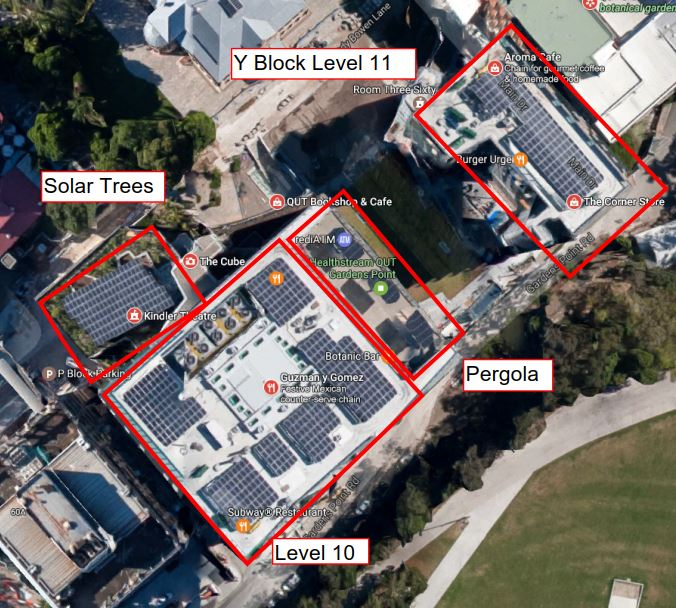
\includegraphics[width=100mm]{images/metering/meteo/pblock-map}\hspace*{\fill}
	\caption{QUT Map Markup with PV Sections} 
	\label{fig:qut-map-pv-markup}
\end{figure}

\paragraph{}
The main page provides an intuitive summary of the modules to provide information on the life of the installation shown below in Figure \ref{fig:qut-lvl10-meteo-summary}. This image was taken at April 15, 2017 for the P Block Level 10 and shows the existing returns that the specific installation has provided. Although the financial information is useful, installations of PV will vary in the financial benefits. The reasoning behind is that different energy providers will allow certain benefits and installations for varying costs. For example, if a client wishes to back-feed (also known as feeding electricity to the grid) certain agreements are required to be made with providers in order to be considered a generator. Additionally, depending on the size of the installation, module manufacturers or distributors may give different discounts per unit reducing the overall capital outlay and reducing the return on investment.       

\begin{figure}[H]
	\hfill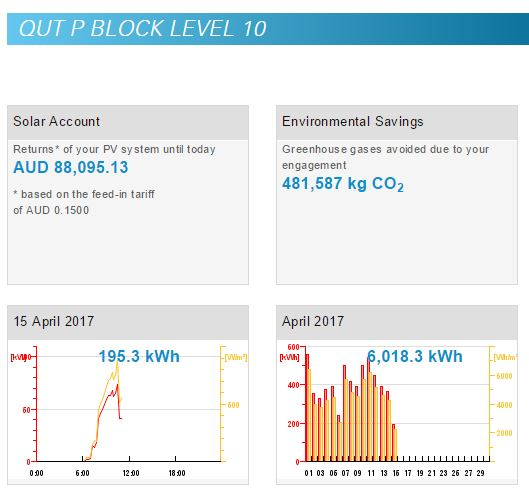
\includegraphics[width = 150mm]{images/metering/meteo/lvl10-summary-page}\hspace*{\fill}
	\caption{QUT Data: P Block Level 10 Meteo Photovoltaic Summary} 
	\label{fig:qut-lvl10-meteo-summary}
\end{figure}

\subsubsection{Power Monitoring Expert}

\paragraph{}
The second monitoring software that QUT Facilities Management allowed access to is Power Monitoring Expert v8.0. This will be used to provide an insight into the load demands of the building that would impact design. Figure \ref{fig:qut-summary-dashboard} outlines the Garden's Point Electricity Metering system. The data is access through a interface closely linked with the single line diagrams of buildings including main switchboards (MSBs), distribution boards (DBs) and transformers. This information is critical to understanding optimal power system design.   

\begin{figure}[H]
	\hfill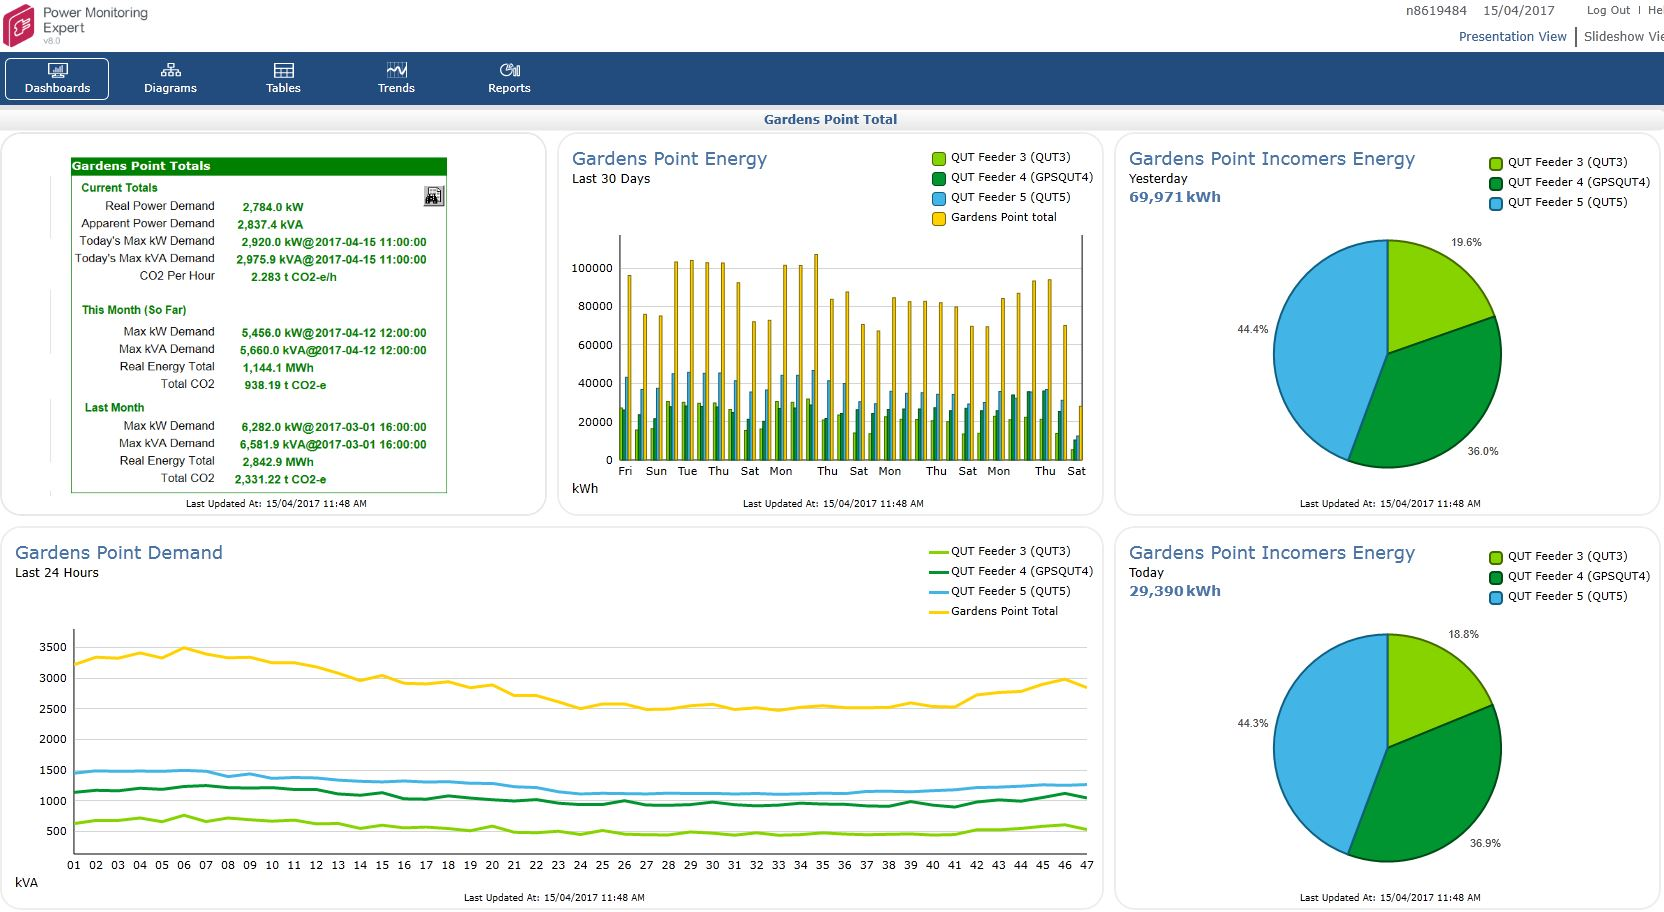
\includegraphics[width = 150mm]{images/metering/pme/summary-dashboard}\hspace*{\fill}
	\caption{QUT Data: Power Monitoring Expert Dashboard} 
	\label{fig:qut-summary-dashboard}
\end{figure}

\paragraph{}
The EMS system additionally outlines how the PV system at QUT operates and what power it generates. The solar panels act as a load reducing generator rather than direct appliance powering. During the day the panels generate electricity and with a regulator and converter combination the DC generated power is converted to AC and fed into the University's power systems. The benefit of utilising the equipment in this way is that it reduces peak consumption which is when electricity prices are highest. The major difference between this design and the one which this project seeks to design is the panels will be directly powering loads.

\newpage

\subsubsection{Useful Data Interpretation}

\paragraph{}
This section outlines the useful data extracted from the two metering systems. The initial task was to analyse all that was available and collate what can be used to produce a more accurate design. With the quantity of data available it was vital to ensure the scope was kept in mind in order to avoid analysing data for no useful reason. 

\paragraph{Photovoltaic Breakdown}
~\\
QUT P Block Level 10 (the same as Figure \ref{fig:qut-lvl10-meteo-summary}) was chosen as a model to analyse the modules, inverters and power quantities produced. Table \ref{table:qut-pblock-lvl10-pv-breakdown} shows the breakdown of the 405 panel and 101.31\,kWp installation. The specific models of module that was installed were the Suntech STP250-20/Wd which are a commercially available and average priced mono-crystalline 250\,W panel. Additionally, there were two variants of the same model inverter installed. These are the 3.6\,kW and 10\,kW versions of the Power-One PVI OUTD/S.        

\begin{table}[H]
	\centering
	\begin{tabular}{|l|l|l|l|l|}
		\hline
		\multicolumn{1}{|c|}{\textbf{Section}} & \multicolumn{1}{c|}{\textbf{Area (\si{m^2})}} & \multicolumn{1}{c|}{\textbf{Peak Power (kWp)}} & \multicolumn{1}{c|}{\textbf{Inverter}} & \multicolumn{1}{c|}{\textbf{Arrays and Size}} \\ \hline
		1                                      & 25                                 & 3.75                                           & 1 x PVI-3.6                            & 1 x 15                                        \\ \hline
		2                                      & 50                                 & 7.5                                            & 1 x PVI-10.0                           & 2 x 15                                        \\ \hline
		3                                      & 139                                & 21.02                                          & 1 x PVI-10.0                           & 1 x 56 \& 1 x 28                              \\ \hline
		4                                      & 330                                & 50.04                                          & 5 x PVI-10.0                           & 1 x 140 \& 1 x 60                             \\ \hline
		5                                      & 38                                 & 5.75                                           & 1 x PVI-5000                           & 1 x 11 \& 1 x 12                              \\ \hline
		6                                      & 41                                 & 6.25                                           & 1 x PVI-6000                           & 1 x 12 \& 1 x 13                              \\ \hline
		7                                      & 46                                 & 7.00                                           & 1 x PVI-6000                           & 2 x 14                                        \\ \hline
		\multicolumn{1}{|c|}{\textbf{TOTAL}}   & \multicolumn{1}{c|}{\textbf{669}}  & \multicolumn{1}{c|}{\textbf{101.31}}           &                                        &                                               \\ \hline
	\end{tabular}
\caption{QUT P Block Level 10 Photovoltaic Array Installation}
\label{table:qut-pblock-lvl10-pv-breakdown}
\end{table}

\paragraph{Photovoltaic Production Data}
~\\
This information is essentially useless without the production data. This monitoring system can provide and graphically represent the production over custom periods. To get accurate readings for Brisbane, Queensland (the location of the proposed system) the entire year of 2016 was assessed to give an accurate represented of predicted production capabilities. Table \ref{table:qut-pv-lvl10-2016} outlines the figures exported by Metero and Figure \ref{fig:qut-pv-lvl10-2016} shows the graphical representation of the output as well as irradiance. 

\paragraph{}
An industry rule of thumb is that in Brisbane, production from a pv installation can receive 1,500\,kWh per kWp. This is only an assumed value but is a guide that can be used for quick approximations. The first consideration was whether the P Block values followed this rule as to assess whether it could be used for future assumptions and design drafting. Table \ref{table:qut-pblock-lvl10-pv-breakdown} shows that the peak power of the entire system is 101.31\,kWp. Following the before mentioned assumption, it could be predicted that over the course of a year, approximately 101.31 x 1500\,kWp will be produced (151,965\,kWp). Table \ref{table:qut-pv-lvl10-2016} below shows the actual metered values for 2016 coming to 157,330.63\,kWp indicating the assumption is quite accurate.   

\begin{table}[H]
	\centering
	\begin{tabular}{|l|c|c|c|}
		\hline
		\multicolumn{1}{|c|}{\textbf{Month}} & \textbf{\begin{tabular}[c]{@{}c@{}}Energy Per Month\\  (kWh)\end{tabular}} & \textbf{\begin{tabular}[c]{@{}c@{}}Energy Per Day \\ (kWh)\end{tabular}} & \textbf{\begin{tabular}[c]{@{}c@{}}Irradiance \\ (kWh/\textbf{\si{m^2}})\end{tabular}} \\ \hline
		\textit{January}                     & 15,360.13                                                                  & 495.49                                                                   & 179.68                                                                                   \\ \hline
		\textit{February}                    & 14,491.13                                                                  & 499.69                                                                   & 170.18                                                                                   \\ \hline
		\textit{March}                       & 12,987.95                                                                  & 418.97                                                                   & 151.04                                                                                   \\ \hline
		\textit{April}                       & 11,976.68                                                                  & 399.22                                                                   & 137.84                                                                                   \\ \hline
		\textit{May}                         & 10,820.50                                                                  & 349.05                                                                   & 126.70                                                                                   \\ \hline
		\textit{June}                        & 7,869.84                                                                   & 262.33                                                                   & 87.05                                                                                    \\ \hline
		\textit{July}                        & 9,704.54                                                                   & 313.05                                                                   & 107.52                                                                                   \\ \hline
		\textit{August}                      & 12,199.19                                                                  & 393.52                                                                   & 136.48                                                                                   \\ \hline
		\textit{Setpember}                   & 12,817.71                                                                  & 427.26                                                                   & 145.39                                                                                   \\ \hline
		\textit{October}                     & 15,481.07                                                                  & 499.39                                                                   & 196.98                                                                                   \\ \hline
		\textit{November}                    & 17,327.80                                                                  & 577.59                                                                   & 203.86                                                                                   \\ \hline
		December                             & 16,294.04                                                                  & 525.61                                                                   & 193.98                                                                                   \\ \hline
		\multicolumn{1}{|c|}{\textbf{TOTAL}} & \textbf{157,330.63}                                                        & \textbf{}                                                                & 1,836.68                                                                                 \\ \hline
	\end{tabular}
	\caption{QUT Data: P Block Level 10 2016 Production Summary Table}
	\label{table:qut-pv-lvl10-2016}
\end{table}

\begin{figure}[H]
	\hfill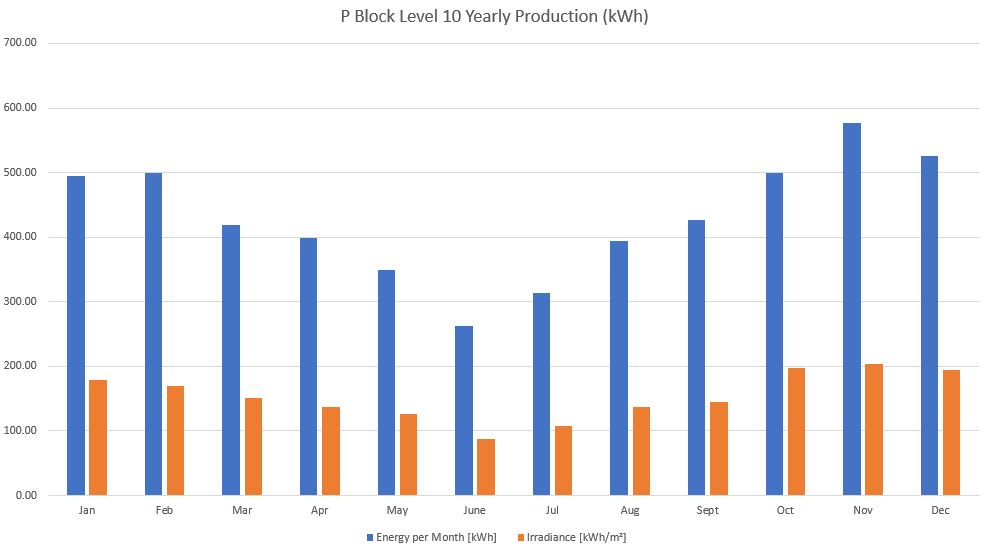
\includegraphics[width = 150mm]{images/metering/meteo/p-block-lvl10-yearly-production}\hspace*{\fill}
	\caption{QUT Data: P Block Level 10 2016 Production Summary Graph} 
	\label{fig:qut-pv-lvl10-2016}
\end{figure}  

\paragraph{Useful Conclusions}
~\\
An important conclusion to make from this data is that the 405 panel installation with a 101.31\,kWp over 1 year can produce 157,330.63\,kWh. A simple calculation therefore gives us a loose approximation that each panel, in Brisbane over 1 year will produce 388.4\,kWh. This can be used to calculate the demand required for the power systems to establish a system for AC powering and then conversions for DC. There are a few key characteristics and assumptions that will be required:
\newline
\begin{itemize}[noitemsep,nolistsep]
	\item Real Power = Apparant Power * Power Factor
	\item kWh is what electricity bills are charged in
	\item kVA is what max demand calculations are based on
	\item DC Power Production is approximately 7\% higher than AC from these modules (from System Advisor Model)
\end{itemize} 

\newpage

\paragraph{Power Monitoring Expert}
~~\\
Similar to the photovoltaic metering system, the Power Monitoring Expert (PME) product that QUT uses provides a large amount of data that needs to be analysed. PME also shows summary pages of the separate locations on both the Garden's Point as well as breakdowns to electrical infrastructure as represented in Figure \ref{fig:qut-pme-pblock-summary}. 

\begin{figure}[H]
	\hfill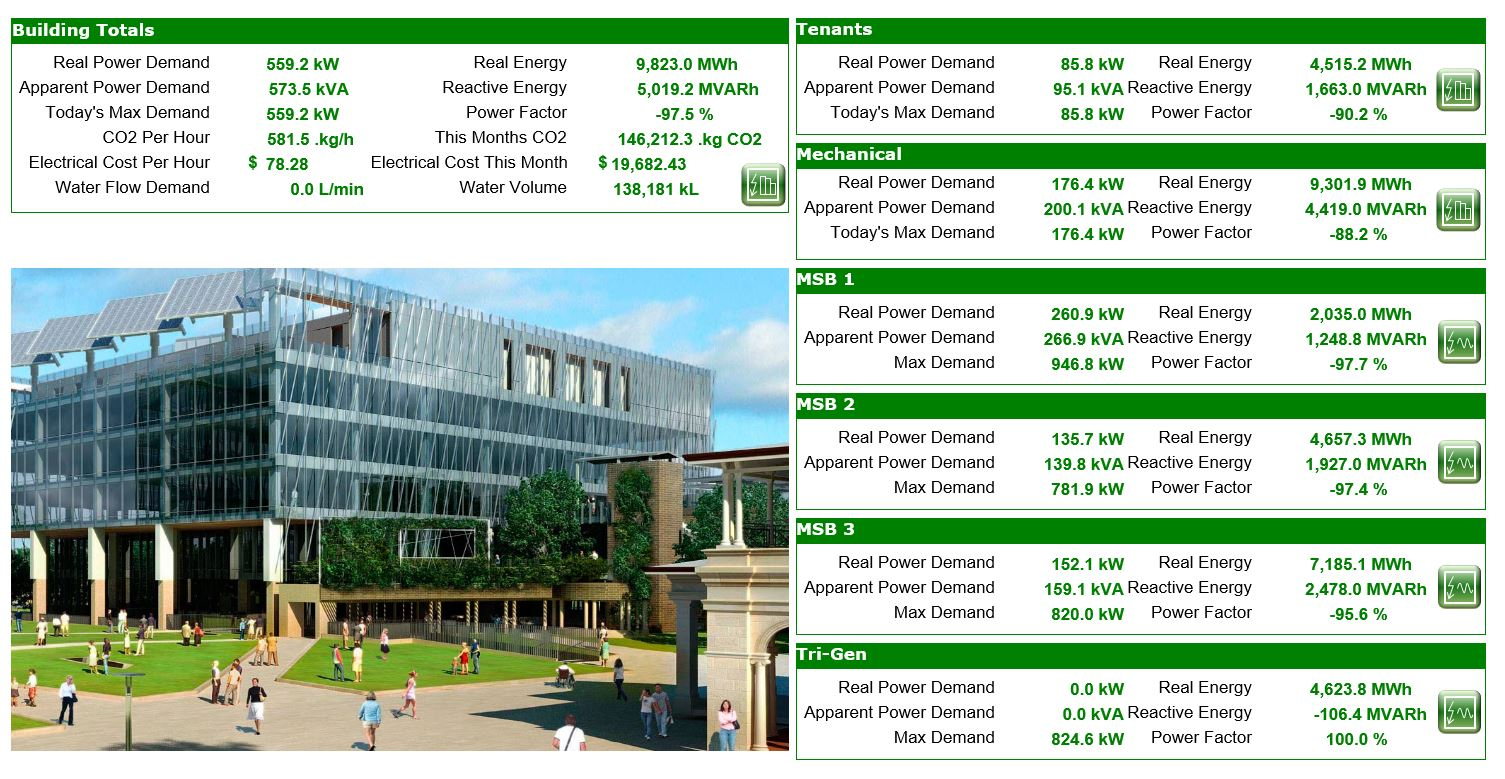
\includegraphics[width = 150mm]{images/metering/pme/pme-p-block-summary-page}\hspace*{\fill}
	\caption{QUT Data: P Block Power Summary (12AM - April 16 2017)} 
	\label{fig:qut-pme-pblock-summary}
\end{figure} 

\paragraph{Data Extraction}
~~\\
What data needs to be exported? To solve this the model for Level 7 of P Block as levels 7, 8 and 9 have the highest density of office rooms per level for the building. Figure \ref{fig:project-model-pblock-lvl7} shows the lighting layout for level 7 and the quantity of luminaires installed. Additionally, it separates the floor plan onto the different distribution boards DB-P-7A, DB-P-7B and DB-P-7C. Following the floor plan, the building's power systems must be separated to understand where the power for the lighting comes from so the correct infrastructure can be observed within the metering system. The extract from the single line diagram is also shown in Figure \ref{fig:project-model-pblock-lvl7-sld-extract} showing that each DB is split to separate power and lighting metering units. This will be integral to estimating the required electricity for lighting loads.      

\begin{figure}[H]
	\hfill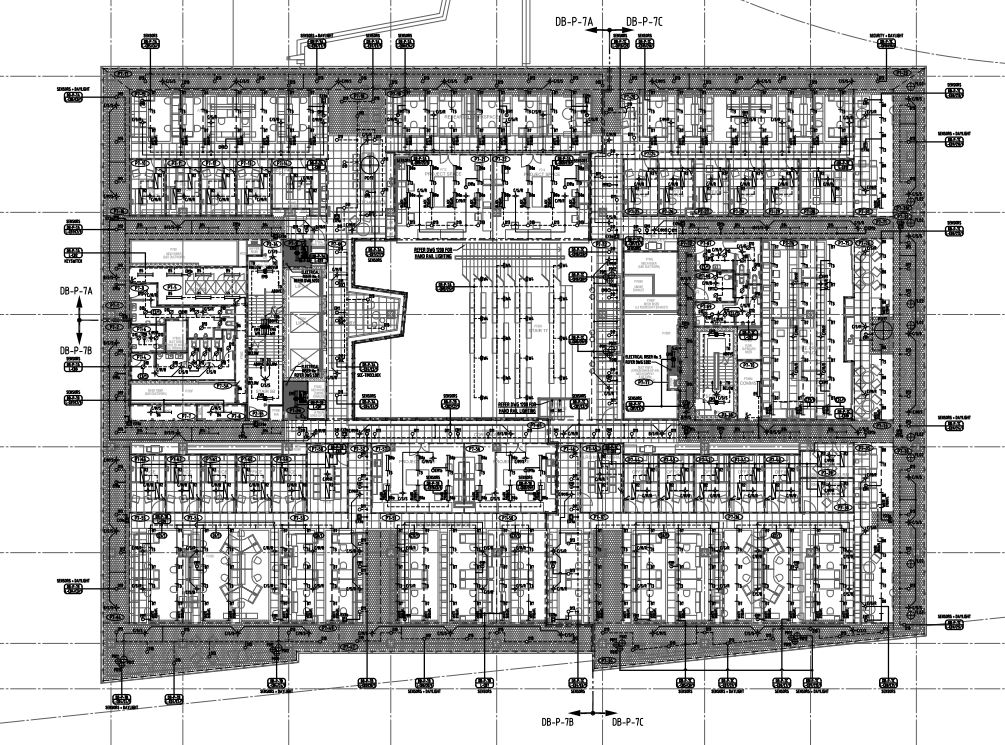
\includegraphics[width = 120mm]{images/project-model/qut-lvl7-lighting}\hspace*{\fill}
	\caption{QUT Layout: P Block Level 7 Lighting Layout} 
	\label{fig:project-model-pblock-lvl7}
\end{figure}

\begin{figure}[H]
	\hfill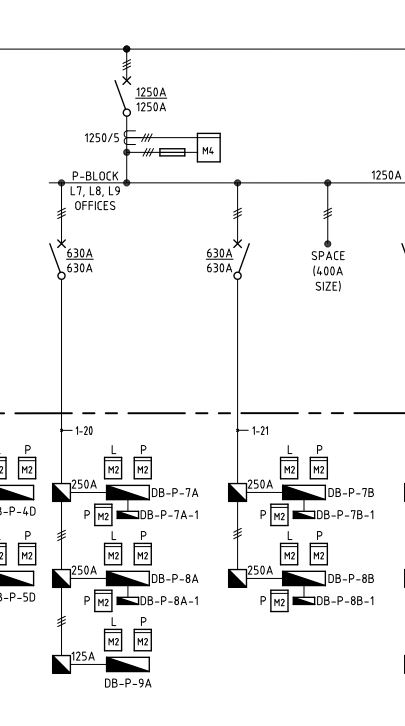
\includegraphics[width = 50mm]{images/project-model/qut-lvl7-sld-extract}\hspace*{\fill}
	\caption{QUT Layout: P Block Level 7 Single Line Diagram Extract} 
	\label{fig:project-model-pblock-lvl7-sld-extract}
\end{figure}

\paragraph{}
The three DBs were found in Power Monitoring Expert for both the power and lighting meters. This was exported into a report and excel spreadsheet. The report is not attached with this paper due to the additional 600 pages it would require. Instead, the data is analysed and summarised below. The metered produced data in 15 minute increments. This means manipulation was required in order to remove a useful conclusion. Figure \ref{fig:pblock-lvl7-monthly-kw} is the graph of the average monthly lighting demand for level 7 over all 3 DBs. It can be seen that there are only minor differences along each month drawing the conclusion that time of year has a negligible effect on the lighting consumption of this floor.  

\begin{figure}[H]
	\hfill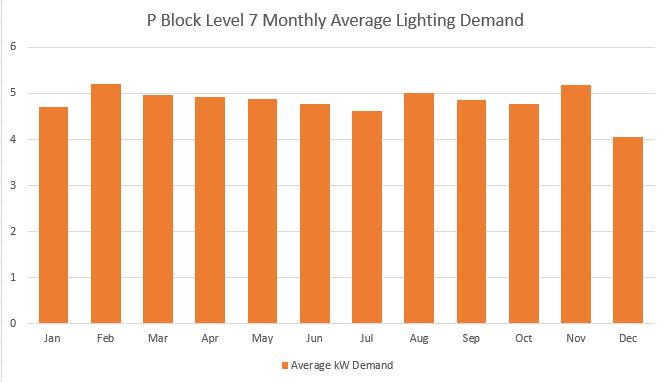
\includegraphics[width = 150mm]{images/metering/pme/pblock-lvl7-monthly-kw}\hspace*{\fill}
	\caption{QUT Data: P Block Level 7 Lighting Demand (kW)} 
	\label{fig:pblock-lvl7-monthly-kw}
\end{figure}  

\paragraph{}
Although this information is useful for the production vs consumption curves however from a energy billing perspective, the kWh needs to be known rather than kW since this is what energy providers charge for. This will also allow for further financial analysis to be completed. Thankfully it is a very simple conversion of P(kWh) = P(kW) * time(h). Because the data is being provided in 15 minute intervals, the kW value must be multiplied by 0.25 to solve for kWh. The graph shown in Figure \ref{fig:pblock-lvl7-monthly-kwh} shows the monthly breakdown of the calculated kWh values. It should ne noted it is just a scaled down replication of the kW graph.    

\begin{figure}[H]
	\hfill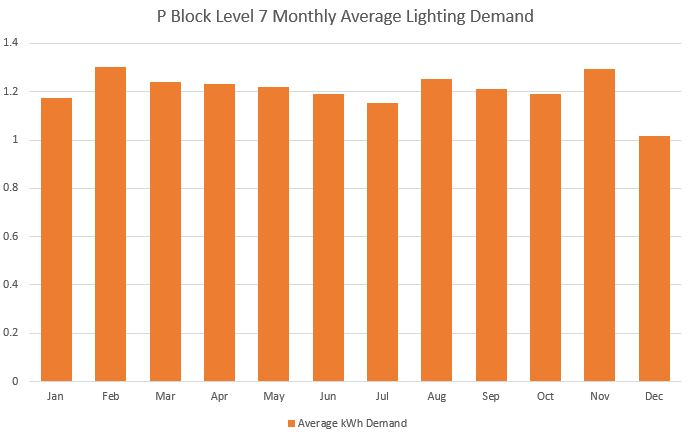
\includegraphics[width = 150mm]{images/metering/pme/pblock-lvl7-monthly-kwh}\hspace*{\fill}
	\caption{QUT Data: P Block Level 7 Lighting Demand (kWh)} 
	\label{fig:pblock-lvl7-monthly-kwh}
\end{figure} 

\paragraph{}
Due to this finding, it was beneficial to model the average daily lighting consumption over each metering period. Figure \ref{fig:pblock-lvl7-15-minute} below shows the consumption curve and can be used to compare against production to determine feasibility.  

\begin{figure}[H]
	\hfill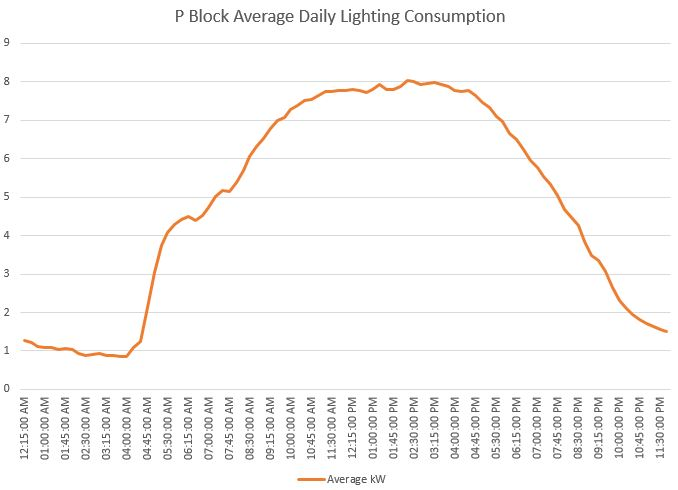
\includegraphics[width = 150mm]{images/metering/pme/pblock-lvl7-daily-avg-kw}\hspace*{\fill}
	\caption{QUT Data: P Block Level 7 15-Minute Interval Lighting Demand (kW)} 
	\label{fig:pblock-lvl7-15-minute}
\end{figure}

\paragraph{Lighting Considerations - Sensors}
~\\
Although the previous data sets in Figure \ref{fig:pblock-lvl7-monthly-kwh} and Figure \ref{fig:pblock-lvl7-15-minute} are highly useful, due to the use of the building being assessed, certain considerations must be taken for the data. In this scenario, the building is within a University requiring different demands. For example, standard business hours in Brisbane are between 8:30\,AM and 5:30\,PM but Figure \ref{fig:pblock-lvl7-15-minute} shows that consumption begins earlier than this and finishes later. Additionally, lighting consumption never hits 0 implying that, on average, there are always lights on. Additionally, upon analysis of the building documentation, P Block has lighting control systems including personnel sensors, light level sensors and illuminance sensors indicating that people are likely in the room at all hours driving the average consumption above 0. Additionally, as a public space it is likely that every light in the building is turned off at any stage. 

\paragraph{Lighting Considerations - Periods}
~\\
In addition to the sensors, a University building will have varied consumption depending on the time of year. This is due to:
\newline
\begin{itemize} [noitemsep]
	\item During study period (In-Semester)
	\item Out of study period (Non-Semester)
	\item Weekday
	\item Weekend
\end{itemize}

All these factors must be considered in the final design. The assessed data could be potentially useless if the varying periods of increased people traffic within the building. Figure \ref {fig:pblock-lvl7-15-minute-detailed} represents the new graphical representation of consumption comparing various yearly period factors and finding the 15\,minute average. Additionally, standard business hours have been marked by the two vertical red lines. This area begins at 8:30\,AM and finishes at 5:30\,PM.  

\begin{itemize} [noitemsep]
	\item Average In-Semester (Dark Blue)
	\item Average Entire Year (Orange)
	\item Average Weekend (Grey)
	\item Average Weekday (Yellow)
	\item Average Out of Semester (Light Blue)
\end{itemize}

\begin{figure}[H]
	\hfill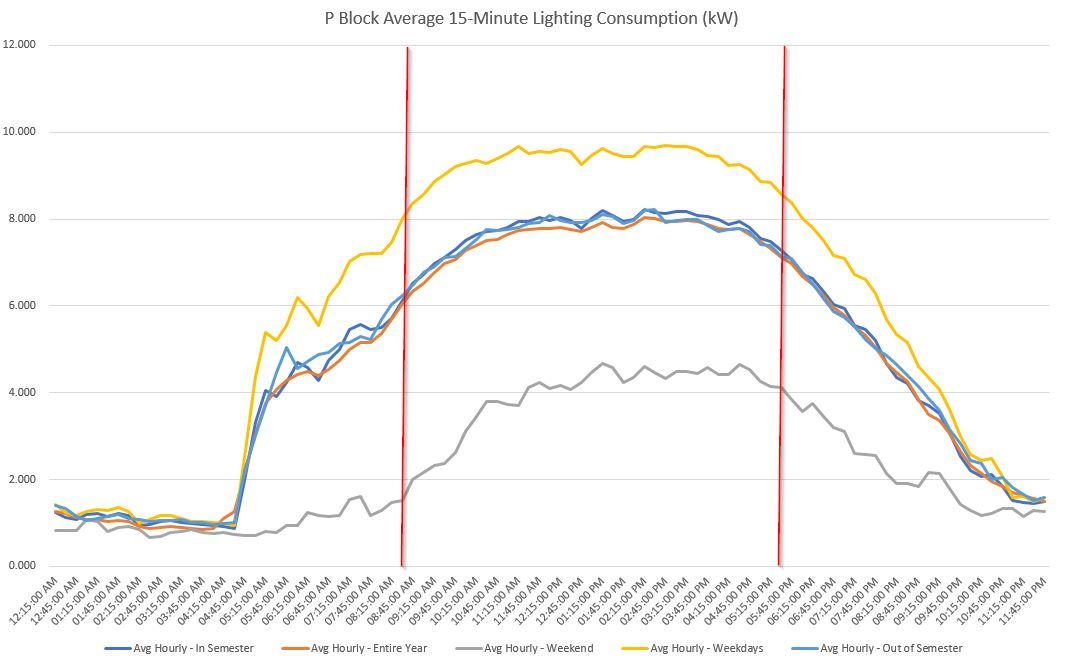
\includegraphics[width = 150mm]{images/metering/pme/pblock-lvl7-daily-avg-kw-detailed}\hspace*{\fill}
	\caption{QUT Data: P Block Level 7 Detailed 15-Minute Interval Lighting Demand (kW)} 
	\label{fig:pblock-lvl7-15-minute-detailed}
\end{figure}
  
\paragraph{Useful Conclusions}
~\\
Analysing the graph above, the only variables that impact the consumption significantly is whether it is during the week or a weekend. It can be seen that weekend consumption does not increase at the same rate and the maximum is approximately 50\% less. Because this data is being used for the modelling of a ``real world" corporate building, the spikes of consumption at 5\,AM will be reduced so the gradiant of the curve begins increasing at 6:30\,AM and shifts to minimum at 7\,PM. The extended hours are to account for employees who arrive at work early and leave later.  Additionally, offices generally do not consume on the weekends meaning that the Yellow line from Figure \ref{fig:pblock-lvl7-15-minute-detailed} is the most accurate. Using this more accurate consumption information as well as assumptions based on Brisbane corporate office buildings, a custom consumption curve has been created in Figure \ref{fig:data-lighting-consumption-custom}.     

\begin{figure}[H]
	\hfill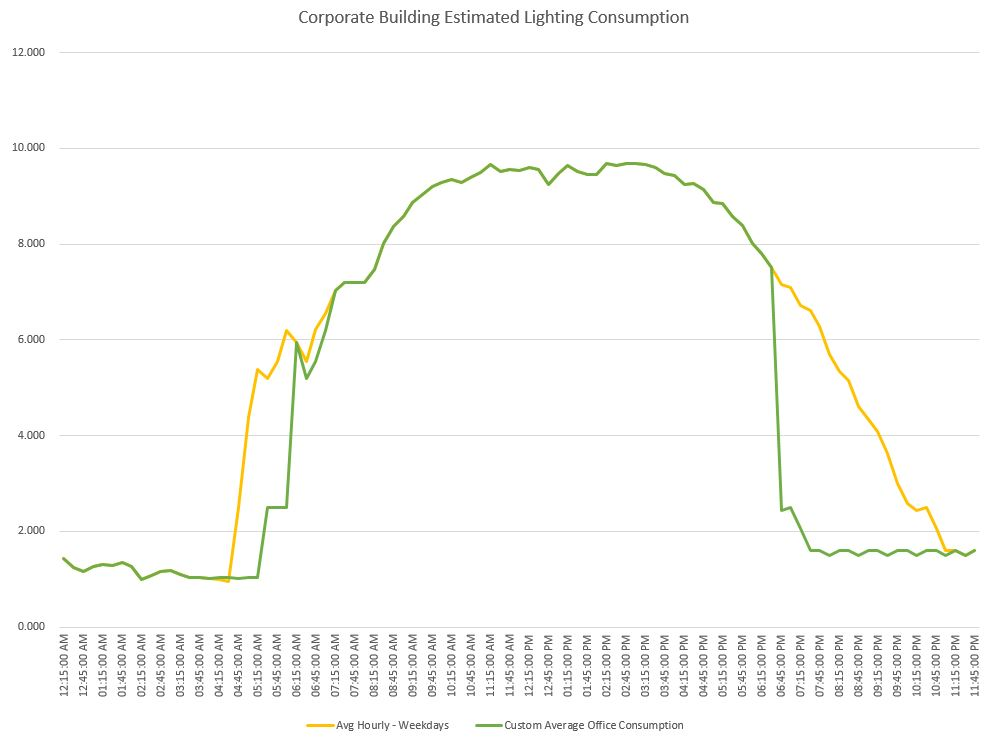
\includegraphics[width = 150mm] {images/metering/pme/corporate-building-lighting-consumption-custom}\hspace*{\fill}
	\caption{Custom Corporate Office Lighting Consumption Comparison} 
	\label{fig:data-lighting-consumption-custom}
\end{figure}
 
\newpage